\documentclass{cmspaper}
\begin{document}

%==============================================================================
% title page for few authors

\begin{titlepage}

% select one of the following and type in the proper number:
%   \cmsnote{2006/000}
  \internalnote{2006/000}
%  \conferencereport{2005/000}
   \date{1 April 2006}

  \title{Digitization Simulation in CMS Calorimetry}

  \begin{Authlist}
     F.~Cossutti\Iref{INFN}, P.~Govoni\Iref{INFN}, C.~M.~Kuo, J.~Mans\Iref{Minnesota}, R.~Wilkinson\Iref{Caltech}
       \Instfoot{INFN} {Instituto National de Fisica Nuclear, Somewhere, Italy}
       \Instfoot{Minnesota} {University of Minnesota, Minneapolis, MN, USA}
       \Instfoot{Caltech}{California Institute of Technology, Pasadena, CA, USA}
  \end{Authlist}

% if needed, use the following:
%\collaboration{Flying Saucers Investigation Group}
%\collaboration{CMS collaboration}

  %\Anotfoot{a}{On leave from prison}
  %\Anotfoot{b}{Now at the Moon}

  \begin{abstract}
    We describe the CMSSW implementation of the digitization step of
    Monte Carlo simulation for the ECAL, HCAL, and preshower.
  \end{abstract} 

\note{Preliminary version}
  
\end{titlepage}

\setcounter{page}{2}%JPP

%==============================================================================
% title page for many authors
%
%\begin{titlepage}
%  \internalnote{2005/000}
%  \title{CMS Technical Note Template}
%
%  \begin{Authlist}
%    A.~Author\Iref{cern}, B.~Author\Iref{cern}, C.~Author\IAref{cern}{a},
%    D.~Author\IIref{cern}{ieph}, E.~Author\IIAref{cern}{ieph}{b},
%    F.~Author\Iref{ieph}
%  \end{Authlist}
%
%  \Instfoot{cern}{CERN, Geneva, Switzerland}
%  \Instfoot{ieph}{Institute of Experimental Physics, Hepcity, Wonderland}
%  \Anotfoot{a}{On leave from prison}
%  \Anotfoot{b}{Now at the Moon}
%
%  \begin{abstract}
%    This is a template of a CMS paper, written in LaTeX,
%    processed with {\it cmspaper.sty} style.
%    It is based on the {\it cernart.sty} and {\it articlet.sty} styles.
%    There are two versions of the title page.
%    The current one is designed for many authors.
%    The one on the previous page is for few authors.
%    Just delete the one which you do not need.
%  \end{abstract} 
%  
%\end{titlepage}
%
%==============================================================================

\section{Introduction}


\section{Calorimetry Framework (CaloSimAlgos)}

The SimHits are the output of the CMSSW GEANT4 simulation
\subsection{SimHits}

The SimHits are the output of the CMSSW GEANT4 simulation, and represent energy deposits in
detector volumes.  They are stored in the following branches of the event's ROOT file:

\begin{verbatim}
 PCaloHits_SimG4Object_EcalHitsEB
 PCaloHits_SimG4Object_EcalHitsEE
 PCaloHits_SimG4Object_EcalHitsES
 PCaloHits_SimG4Object_HcalHits
\end{verbatim}

The SimHit objects themselves have four fields:
\begin{itemize}
\item sim track ID
\item Detector ID
\item energy
\item time
\end{itemize}

The sim track ID refers to the generated particle, and the detector ID
refers to the calorimeter cell, according to the numbering scheme
described in~\ref{roadmap}.  The time represents the time-of-flight,
with zero being the interaction time.  Pileup hits have their
times adjusted by the mixing module to correspond to an earlier or
later bunch crossing.  The energy represents different
quantities in different subsystems.  In ECAL and preshower, it is the
energy deposit, in GeV.  For Hcal Forward, it is the number of photoelectrons
produced.  For the other HCAL subsystems, it is the sampled energy,
which is a fixed fraction of the incident energy, as shown in table~\ref{sampling}.

    \begin{center}
      \begin{tabular}{|l|c|c|} \hline
       \label{sampling}
         SimHit Subdetector & meaning of ``energy()'' & Sampling Factor \\ \hline
         ECAL & Full incident energy & 1. \\ 
         Preshower & Full incident energy & 1. \\ 
         HCAL (HB \& HE) & Sampled energy & 117.\\
         HCAL (HO) & Sampled energy & 217. \\ 
         HCAL (HF1) & Photoelectrons & 2.84 \\
         HCAL (HF2) & Photoelectrons & 2.09 \\ \hline
      \end{tabular}
    \end{center}

Note that SimHits have no information about their position
within the detector, so no effects such as delays or attenuation
based on position within the cell are possible.

To give an idea of what SimHits look like, a typical 100 GeV central electron
will create N SimHits across X crystals, and a typical 100 GeV central charged
pion creates 85 Hcal SimHits across X cells.


\subsection{Hit Correction}

We allow an interface, CaloVHitCorrection, to apply corrections to the SimHits before
they are processed.  This is currently used by the HCAL to implement
time slewing.  

Time slew is observed in the HCAL electronics, whereby smaller signals get delayed
by up to 10 ns.  This effect is modeled by adding a delay to the SimHit time,
based on the hit energy.  This may exaggerate the effect, however,
because, as mentioned in the previous section, a signal can have many low-energy
SimHits.  We plan to introduce a mechanism to merge SimHits in 
each cell if they arrive within a nanosecond of each other, so the
combined SimHits will more accurately correspond to the final
signal amplitude.

The HCAL time slew is shown in figure~\ref{fig:slew}, for three QIE bias settings: slow, medium, and fast.  HO uses the slow (and lower noise) setting, while the other subsystems use the medium setting.

\begin{figure}[hbtp]
  \begin{center}
    \resizebox{10cm}{!}{\includegraphics{slew.eps}}
    \caption{Time delay as a function of signal size, in fC, for QIE bias settings of slow (top), medium, and fast.  HO uses the slow setting, while the other subsystems use the medium setting.}
    \label{fig:slew}
  \end{center}
\end{figure}

\subsection{Photostatistics}

From the SimHit energy, the mean number of photoelectrons is
fist found by multiplying by a constant found in the CaloSimParameterMap, the photomultiplierGain().
A Poisson random number is thrown to obtain the amplitude of 
the charge pulse.  The default values of this constant are shown
in table~\ref{photostat}

\begin{center}
      \begin{tabular}{|l|c|} \hline
       \label{photostat}
         Subdetector & SimHit to Photoelectrons factor  \\ \hline
         ECAL (EB) & 2250  pe/GeV \\
         ECAL (EE) & 1800 pe/GeV \\
         Preshower & (not needed) \\
         HCAL (HB,HE) & 2000 pe/ sampled GeV  \\
         HCAL (HB,HE) & 4000 pe/ sampled GeV  \\
         HCAL (HF) & (not needed)  \\ \hline
      \end{tabular}
\end{center}


\subsection{Shaping}

The next step for each SimHit is to be converted into an analog signal,
using a pulse shape interface from CaloVShape.  These analog signals
are summed and stored in the CaloSamples class.  The samples are assumed
to represent 25 ns spacing.

The timing for these signals is determined by a field in the CaloSimParameterMap,
the PeakBin.  In order to position the peak in the center of this time bin, we correct for the signal peaking
time and speed-of-light
propagation from the interaction at t=0, as well as allowing an additional time phase
adjustment.  The timing parameters are shown in table~\ref{timing}

\begin{center}
      \begin{tabular}{|l|c|c|c|c|} \hline
       \label{timing}
         Subdetector & Shaping Class & Shaper Peaking Time (ns) & Peak Bin & Timing Adjustment (ns) \\ \hline
         ECAL & EcalShape & 47.6 & 5/10 & 0 \\ 
         Preshower & ESShape & 20  & 2/3 & 0 \\ 
         HCAL (HB,HE,HO) & HcalShape & 14  & 5/10 & -2 \\
         HCAL (HF) & HFShape & 2 & 4/6 & -6 \\ \hline
      \end{tabular}
\end{center}

\section{Calibration Databases}

The digitization is being designed to get whatever parameters it can from calibration 
and conditions databases.  This will allow more realistic simulation of the actual
detector: we can make hot channels hot, and noisy channels noisy.  It also lets
us exercise the calibration algorithms in a "calibration challenge", where data
will be simulated with a hidden set of pedestals and gains, which the physics
groups must derive.

The default mode of operation will be use a calibration interface, but with
simple parameters, constant across all channels.  These parameters are hardcoded
now, but could easily be made configurable.  The default pedestals and gains
are shown in table~\ref{calibrations}.

\subsection{Pedestals and Gains}
\begin{center}
      \begin{tabular}{|l|c|c|c|c|c|} \hline
       \label{calibrations}
         Subdetector & Scale (LSB) & Pedestal & Pedestal Width & Gain & Gain Width \\ \hline
         EB Gain 12 & 35 MeV & 198.8 ADC & 1.10 ADC (40 MeV) & 12. & 0.2\%\\ 
         EB Gain  6 & 70 MeV & 199.4 ADC & 0.90 ADC  & 6. & 0.2\%\\ 
         EB Gain  1 & 420 MeV & 201.8 ADC & 0.62 ADC  & 1. & 0.2\%\\
         ECAL (EE) & XX MeV & 200 ADC ?  & 4 ADC? (150 MeV) & 1.  & 0.2\%\\ 
         Preshower &  XX MeV &  1000 ADC  & 3 ADC  & 9 ADC/keV (?) & 0. \\ 
         HCAL (HB, HE, HO) & 1 fC & 0.75 GeV  (5 ADC) & 0.1 GeV (0.56 ADC) &  0.177 GeV/fC (x2000 amp.) & 0\\
         HCAL (HF1) & 1 fC & 0.75 GeV (2 ADC) & 0.14 GeV (0.3 ADC)&  0.48 GeV/fC  & 0  \\ \hline
      \end{tabular}
\end{center}

\subsubsection{ECAL}

\subsubsection{HCAL}

The pedestals and gains for the HCAL are accessed not only by readout channel, but individually for each of the four readout capacitors in the channel.  These capacitors are accessed in a round-robin sequence.  One of the four is randomly picked to be the starting capacitor, and the starting capacitor number is kept consistent throughout the subdetector in the event.

\section{Encoding}

All Calorimetry subdetectors except Preshower define a non-linear scheme through which
the analog signal amplitudes are packed into 16-bit data fields.  
The encoding algorithms are described below:

\subsection{ECAL}

The ECAL samples come from a MultiGainPreAmplifier (MGPA), which has gains of 1, 6, and 12.
The gain is encoded with two bits, while the ADC value is encoded with twelve bits.
Each ADC count is hardcoded now to represent 35 MeV in the barrel and 60 MeV in the endcap,
although we plan to move these numbers into a conditions database.

We include a hysteresis effect in gain switching: we stay at the higher
gain for five samples after it has been activated.

\subsection{Preshower}

The default mode of operations in the preshower is 
to use a gain of 9 ADC counts per keV, up to a saturation
of 4095 counts.  A calibration mode is also provided,
with a gain of 50 ADC counts per keV.

\subsection{HCAL}

HCAL encoding is done through an interface to the conditions DB.
The HCAL charge is coded into only seven bits.
These bits represent one fC up to a value of 15 fC,
then switch to two fC per bit up to thirty fC,
switching to progressively coarser granularity, until
a saturation at 10,000 fC.

\section{Zero Suppression}
\subsection{ECAL}
\subsection{Preshower}
\subsection{HCAL}

\section{Trigger Primitives}
\subsection{ECAL}

These are just being implemented now.

\subsection{HCAL}


\section{Unit Tests and Validation}

\subsection{Standalone tests}

\subsubsection{ECAL}

\subsubsection{HCAL}
The HcalDigitizerTest is meant to be a standalone
test of the digitization chain.

We'll start with an example of an incident particle of 100 GeV energy
in the HB.  The sampling factor is 117, so we expect the SimHit
to have 0.855 GeV of energy.

We next convert to photoelectrons, giving 0.855 * 2000 = 1710.
These photoelectrons are subjected to Poisson statistics.
Next they go through the shaping to give a pulse, still in the units
of photoelectrons:

\begin{verbatim}
DetId=1107320961, 10samples
0:0
1:0
2:0
3:0
4:814.103
5:657.711
6:185.86
7:73.7753
8:31.0982
9:13.2264
\end{verbatim}

This pulse is converted to fC by multiplying by the
factor of 0.33 found above.  Next, this analog signal
is encoded, resulting in the following digi:

\begin{verbatim}
(HE 17,1,1) 10 samples  4 presamples
  ADC=4, capid=1, DV
  ADC=4, capid=2, DV
  ADC=4, capid=3, DV
  ADC=4, capid=0, DV
  ADC=58, capid=1, DV
  ADC=54, capid=2, DV
  ADC=33, capid=3, DV
  ADC=21, capid=0, DV
  ADC=14, capid=1, DV
  ADC=9, capid=2, DV
\end{verbatim}

No noise has been added to this digi.  Default running will add noise.

HF behaves similarly, except with a much narrower time peak.
Here are the analog signals for a 100 GeV incident particle,
in the long and short fibers, respectively:

\begin{verbatim}
DetId=1207987969, 6samples
0:0
1:0
2:0
3:35.2
4:0
5:0

DetId=1208004353, 6samples
0:0
1:0
2:0
3:47.8
4:0
5:0
\end{verbatim}

and here are the corresponding (noiseless) digis:

\begin{verbatim}
HF Frames
(HF 30,1,1) 6 samples  3 presamples
  ADC=13, capid=0, DV
  ADC=13, capid=1, DV
  ADC=13, capid=2, DV
  ADC=93, capid=3, DV
  ADC=13, capid=0, DV
  ADC=13, capid=1, DV

(HF 30,1,2) 6 samples  3 presamples
  ADC=13, capid=0, DV
  ADC=13, capid=1, DV
  ADC=13, capid=2, DV
  ADC=93, capid=3, DV
  ADC=13, capid=0, DV
  ADC=13, capid=1, DV
\end{verbatim}

\subsection{Diagnostics}

All subdetectors SHOULD have a module which runs a passive check
check of the digis to see if the pedestals and gains
are implemented correctly.  To test the gains,
these modules compare
the RecHit energies of cells over a threshold
with the summed SimHit energy in the cell, and 
throw errors if the results are farther than
the expected mean.  These modules 


\section{Configurable parameters}

Following is the list of configurable parameters for the system:

\bf{SimCalorimetry/EcalSimProducers/data/ecaldigi.cfi:}

\begin{verbatim}
module ecaldigi = EcalDigiProducer
{
  untracked double simHitToPhotoelectronsBarrel = 2250.
  untracked double simHitToPhotoelectronsEndcap = 1800.
  untracked double photoelectronsToAnalogBarrel = 0.000444444
  untracked double photoelectronsToAnalogEndcap = 0.000555555
  untracked double samplingFactor = 1.
  untracked double timePhase = 47.6683
  untracked int32 readoutFrameSize = 10
  untracked int32 binOfMaximum = 5
  untracked bool doPhotostatistics = true
  untracked bool doNoise = true
  untracked int32 ESGain = 1
  untracked bool doESNoise = true
  untracked double ESNoiseSigma = 3.
  untracked int32 ESBaseline = 1000
  untracked double ESMIPADC = 9.
  untracked double ESMIPkeV = 78.47
}

\end{verbatim}

\bf{SimCalorimetry/HcalSimProducers/data/hcaldigi.cfi:}

\begin{verbatim}
module hcaldigi = HcalDigiProducer
{
  bool doTimeSlew = true
  bool doNoise = true
}
\end{verbatim}

\begin{figure}[hbtp]
  \begin{center}
    \resizebox{3cm}{!}{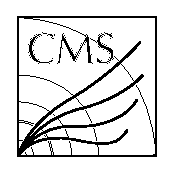
\includegraphics{cmslogo.eps}}
    \caption{Figure inserted by 
      \tt $\backslash$resizebox\{3cm\}\{!\}\{$\backslash$includegraphics\{cmslogo.eps\}\}.}
    \label{fig:ex1}
  \end{center}
\end{figure}

\begin{figure}[hbtp]
  \begin{center}
    \resizebox{5cm}{1cm}{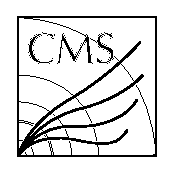
\includegraphics{cmslogo.eps}}
    \caption{Figure inserted by 
       \tt $\backslash$resizebox\{5cm\}\{1cm\}\{$\backslash$includegraphics\{cmslogo.eps\}\}.}
    \label{fig:ex2}
  \end{center}
\end{figure}

Quite often it is convenient to place 2 figures side by side as a single
floating body. An environment {\em 2figures} is provided for that
(see Fig.~\ref{fig:ex3} and \ref{fig:ex4}).

\begin{2figures}{hbtp}
  \resizebox{\linewidth}{0.5\linewidth}{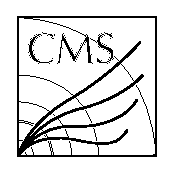
\includegraphics{cmslogo.eps}} &
  \resizebox{\linewidth}{0.5\linewidth}{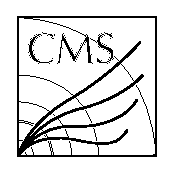
\includegraphics{cmslogo.eps}} \\
%  \resizebox{\linewidth}{!}{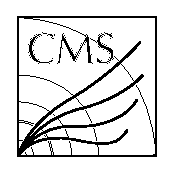
\includegraphics{cmslogo.eps}} &
%  \resizebox{\linewidth}{!}{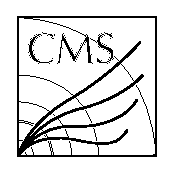
\includegraphics{cmslogo.eps}} \\
  \caption{The left figure}
  \label{fig:ex3} &
  \caption{The right figure}
  \label{fig:ex4} \\
\end{2figures}

%------------------------------------------------------------------------------

\section{Submitting a note}

Please follow the rules and procedures defined on the CMSDOC server, or request them by e-mail to:\begin{center} {\em cmsnotes@cmsdoc.cern.ch} \end{center}

\section{Reference example}

References should be placed at the end of the note 
(see example \cite{NOTE000}).

\begin{thebibliography}{9}
  \bibitem {NOTE000} {\bf CMS Note 2005/000},
    X.Somebody et al.,
    {\em "CMS Note Template"}.
\end{thebibliography}
 
%------------------------------------------------------------------------------
\pagebreak



\end{document}
